\documentclass[11pt]{article}
\usepackage[margin=1in]{geometry}
\usepackage{amsmath,amssymb}
\usepackage{booktabs}
\usepackage{graphicx}
\usepackage{microtype}
\usepackage{natbib}
\usepackage{pgfplots}
\pgfplotsset{compat=1.18}
\usepackage[hidelinks]{hyperref}
\emergencystretch=3em
\Urlmuskip=0mu plus 1mu\relax
\usepackage{xcolor}
\sloppy

\title{\bfseries How Much of a Leaderboard Ranking Survives Its Own Sampling Error?\\
\large A Paired-Resolution Audit of Five AI Benchmarks}
\author{Ilpo V\"a\"at\"ainen\\
\small Independent Researcher\\
\small \texttt{github.com/ipezygj/swebench-rank-audit}}
\date{August 2026}

\begin{document}
\maketitle

\begin{abstract}
A benchmark leaderboard is read as a stopwatch: the rank beside a model is treated as a fact.
Yet every entrant is scored on the \emph{same} items and publishes which it solved, so a
leaderboard is a paired experiment, and its ordering can be tested rather than trusted. We test
each adjacent-rank pair for statistical separability---exact McNemar's test on discordant items for
pass/fail benchmarks, a paired item-bootstrap for scored ones---across five public boards.
On SWE-bench Verified, $129$ of $133$ adjacent ranks are not separable at the $5\%$ level; on MTEB,
$176$ of $180$; on HELM Lite, all $89$ of $89$. The benchmarks are not broken: $88\%$ of \emph{all}
pairs separate cleanly. It is the neighbours they cannot order, and neighbours are what the top of a
table is made of. We derive a resolution bound, $\delta \ge 2.80\sqrt{d/n}$ in the discordance rate
$d$, that predicts which pairs are decidable from a benchmark's size and its near-pair discordance,
validate it on $12{,}739$ pairs
with zero false positives, and use LMArena---which already ships confidence intervals and ties---as a
positive control for what correct reporting looks like. Every figure is recomputed from public data
and passes a self-test suite; the recomputed rates match each official board to its published
precision, with one exception on the Test split, where our rate for one system differs by $1.22$~pp
because its submission file lists $241$ results over $213$ distinct instance ids. We argue that a
board should report the \emph{resolution} of its ranking alongside the ranking, at no additional data
cost.
\end{abstract}

\section{Introduction}
Leaderboards have become the primary product of a benchmark: as \citet{hardt2025} observes, what
practitioners take away is not an evaluation but an \emph{ordering}. A crisp number sits beside each
model and the order is read as settled. But at the crowded top of a board that order is often
softer---an accident of which items happened to be on the test.

This is checkable, because a benchmark scores every entrant on the same items and (for the boards we
study) each entrant publishes exactly which items it solved. The ordering is therefore a
\emph{paired} experiment: to ask whether model $A$ truly outranks the model directly below it, one
need only look at the items on which they \emph{disagree}. Items both solved, or both missed, carry
no information about the order.

Recent work has circled this point from several sides. \citet{huang2025} show that dropping
$0.003\,\%$ of Chatbot Arena's human preferences can change its top-ranked model, by a method built
on influence functions; \citet{singh2025} document undisclosed private testing, selective
disclosure and unequal data access at the top of the same board; \citet{lunardi2025} find that
model rankings stay \emph{relatively} stable under paraphrase even as absolute scores decline
significantly; \citet{miller2024} argues for error bars on eval
numbers, and \citet{wang2025} decomposes eval noise into its item and run components; \citet{zhang2024}
apply Arrow's theorem to ordinal benchmarks and measure a trade-off between a multi-task board's
diversity and its sensitivity to irrelevant changes---a
result about aggregation design that we view as complementary to, rather than implying or implied by,
the finite-sample question we ask here;
\citet{chatzi2024} replace point ranks with rank-sets that carry the uncertainty; and \citet{polo2024} and
\citet{kipnis2024} show, through item-response theory, how few
items actually carry a benchmark's signal. The requirement itself is not new:
\citet{card2020} established for NLP that comparisons need the power to support them, and
\citet{mogstad2024} give simultaneous confidence sets for ranks. We apply that requirement
uniformly to the rank itself, on five public boards, and give a closed form for it from a board's
size and its near-pair discordance. Our contributions:
\begin{enumerate}\itemsep2pt
  \item A single method---exact McNemar for pass/fail, paired item-bootstrap for scores---that tests
  adjacent-rank separability on any board publishing per-item results, applied uniformly to five.
  \item A measured census: most adjacent ranks on four of the five boards are not separable, while
  distant systems separate cleanly, isolating \emph{sampling}, not benchmark quality, as the cause.
  \item A resolution bound $\delta \ge 2.80\sqrt{d/n}$ in the board's size $n$ and its near-pair
  discordance $d$, derived from test power and validated on
  $12{,}739$ pairs with zero false positives, giving the items required to resolve a given gap.
  \item LMArena as a positive control: a board whose confidence intervals and tie-aware ranks already
  report what the others omit, showing the fix is cheap and adopted.
\end{enumerate}

\section{Method}
\label{sec:method}
Let a board rank $m$ systems on $n$ shared items. For a pair $(A,B)$ adjacent in the published order:

\paragraph{Pass/fail benchmarks.} Each item is solved or not. Restricting to the $b+c$ \emph{discordant}
items ($A$ solves and $B$ does not: $b$; the reverse: $c$), the null ``no difference'' is a fair coin,
and we apply the \emph{exact} McNemar test---a two-sided binomial test of $b$ successes in $b+c$
trials against $p=\tfrac12$. Concordant items are excluded because they cannot distinguish the two
systems.

\paragraph{Scored benchmarks.} Each item yields a real score per system. We take a paired bootstrap
over items: resample the $n$ items with replacement, recompute each system's mean, and read the
$95\%$ interval of the paired difference $A-B$; the pair is separated iff that interval excludes zero.
The same resampled items are used for both systems, preserving the pairing.

\paragraph{Aggregate metrics.} When a board ranks by a composite (e.g.\ a mean win rate over
sub-benchmarks), we first \emph{reproduce the published metric} from raw sub-scores and gate on exact
parity before testing, so we test the number the board actually shows.

\paragraph{Self-tests.} No number is reported before a control suite passes: (i) identical systems are
never ordered, in both modes---the negative control; (ii) $60$ planted losses and a uniform score
shift are both detected at $p<10^{-6}$, so the negative control is not passing merely because nothing
is ever detected; (iii) on random data, no pair whose gap clears the bound is left unresolved by
the test. The tool is $\sim\!200$ lines (\texttt{numpy}/\texttt{pandas}/\texttt{scipy}) and ships all
three; a fourth check, that a published Wilson interval is reproduced ($5/10 \to [0.2366, 0.7634]$),
runs in the SWE-bench builder.

\section{Results}
\label{sec:results}
Table~\ref{tab:main} summarises. On \textbf{SWE-bench Verified} ($134$ systems, $500$ instances),
$129$ of the $133$ adjacent-rank pairs are not separable at $5\%$; the top eight systems are statistically
indistinguishable from the \#1 (ranks 1--8, $76.4$--$79.2\%$); the \#1 and \#2 resolve the same count,
and of their $36$ disagreements the split is $18/18$ ($p=1.000$). Yet $7{,}835$ of all $8{,}911$ pairs
($87.9\%$) \emph{are} separated: the board discriminates distant systems well. The median $95\%$ rank
interval is $13$ places wide of $134$; $102$ systems span $\ge 10$ places. The recomputed resolve
rates match the official board for all $133$ systems with a result file (max $|\Delta|=0$).

Extending to all four SWE-bench splits (Table~\ref{tab:splits}) separates cause from artifact. The
full-size \textbf{Test} split ($2{,}294$ items) has a \#1 that leads every one of $2{,}000$ item
bootstraps; on the crowded \textbf{Verified} and \textbf{Lite} splits the leader holds its place in
only $38.3\%$ and $53.6\%$ of them (\texttt{top1\_stability.py}, seed $20260918$). A preregistered prediction---that the undecidable gap scales as $1/\sqrt{n}$ from the Verified
anchor---held for $2$ of $3$ held-out splits (the miss, Multimodal, is explained post hoc by its
small pair count and is reported as a miss).

Two further boards, with no shared data, scoring, maintainers, or outcome type, give the same shape.
On \textbf{MTEB} (eng, v2; $181$ systems $\times$ $41$ tasks, scored), $176$ of $180$ adjacent pairs
are not ordered and four systems are tied with the top. On \textbf{HELM Lite} ($90$ models $\times$
$10$ scenarios, ranked by mean win rate) the win-rate matrix reproduces the published index exactly
(max $|\Delta| = 0.0000$) and then \emph{all} $89$ of $89$ adjacent pairs are not separable---the
extreme case, because ten scenarios cannot order ninety models.

\begin{table}[t]
\centering
\small
\begin{tabular}{lrrcr}
\toprule
Board & Systems & Items & Adjacent pairs \emph{not} separable & All pairs separated\\
\midrule
SWE-bench Verified$^{\dagger}$ & $134$ & $500$ & $129/133$ & $87.9\%$\\
MTEB (eng, v2)     & $181$ & $41$  & $176/180$ & $85.4\%$\\
HELM Lite          & $90$  & $10$  & $\mathbf{89/89}$ & $70.3\%$\\
\midrule
LMArena \emph{(positive control)} & $242$ & 3.0M votes & $238/241$ CIs overlap & ---\\
\bottomrule
\end{tabular}
\caption{Adjacent-rank separability across boards. Distant systems separate ($70$--$88\%$ of all
pairs); neighbours do not. LMArena already reports this via confidence intervals and tie-aware ranks.
$^{\dagger}$~$134$ of the board's $180$ entries publish per-instance results; the census covers those.
MTEB likewise: $181$ of $331$ models report all $41$ tasks.}
\label{tab:main}
\end{table}

\begin{table}[t]
\centering
\small
\begin{tabular}{lrrccr}
\toprule
Split & Systems & Items & Adjacent unclear & \#1 holds under item bootstrap & Largest unclear gap\\
\midrule
SWE-bench Test        & $24$  & $2{,}294$ & $9/23$  & $100.0\%$ & $1.61$ pp\\
SWE-bench Verified    & $134$ & $500$     & $129/133$ & $38.3\%$ & $4.60$ pp\\
SWE-bench Lite        & $84$  & $300$     & $82/83$ & $53.6\%$   & $6.67$ pp\\
SWE-bench Multimodal  & $12$  & $517$     & $11/11$ & not computed & $2.71$ pp\\
\bottomrule
\end{tabular}
\caption{The same test across four SWE-bench splits. Only the large Test split resolves a champion;
the undecidable gap shrinks with $n$, as the preregistered $1/\sqrt{n}$ prediction anticipated.}
\label{tab:splits}
\end{table}

\section{A Resolution Bound}
\label{sec:law}
The pairwise result is not ad hoc. Exact McNemar tests $b/(b+c)$ against $\tfrac12$, and with a gap
$\delta$ in resolve rate and a discordance rate $d$ (the fraction of items on which two systems
differ), $b/(b+c)-\tfrac12 = \delta/2d$. The power of the underlying binomial test then gives
\begin{equation}
\delta \;\ge\; (z_{\alpha/2}+z_{\beta})\,\sqrt{d/n} \;\approx\; 2.80\,\sqrt{d/n}
\qquad (\alpha=0.05,\ \text{power }0.8).
\label{eq:law}
\end{equation}
Two consequences: resolution improves only as $\sqrt{n}$, and---less obviously---it \emph{worsens} as
$\sqrt{d}$: the more two systems differ item-by-item, the harder they are to order at the same
headline gap. Both are readable from published files; $\delta$ is the difference a board already shows, and $d$ is the one no board reports
(Figure~\ref{fig:frontier}).

\begin{figure}[t]
\centering
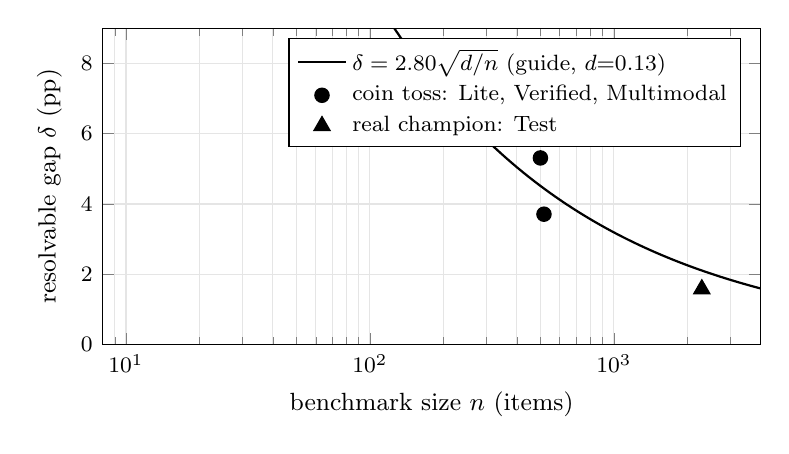
\begin{tikzpicture}
\begin{axis}[
  width=0.82\linewidth, height=5.6cm,
  xmode=log, log basis x=10,
  xlabel={benchmark size $n$ (items)},
  ylabel={resolvable gap $\delta$ (pp)},
  xmin=8, xmax=4000, ymin=0, ymax=9,
  grid=both, grid style={gray!20},
  legend pos=north east, legend cell align=left, legend style={font=\footnotesize},
  tick label style={font=\footnotesize}, label style={font=\small},
]
\addplot[thick, domain=8:4000, samples=120]{2.80*sqrt(0.13/x)*100};
\addlegendentry{$\delta=2.80\sqrt{d/n}$ (guide, $d{=}0.13$)}
\addplot[only marks, mark=*, mark size=2.6pt] coordinates {(300,7.08) (500,5.31) (517,3.71)};
\addlegendentry{coin toss: Lite, Verified, Multimodal}
\addplot[only marks, mark=triangle*, mark size=3.4pt] coordinates {(2294,1.58)};
\addlegendentry{real champion: Test}
\end{axis}
\end{tikzpicture}
\caption{The resolution frontier: the smallest rank gap a benchmark of $n$ items can decide. Each
SWE-bench split is plotted at its own measured near-pair discordance $d$. The three small splits
resolve only $3.7$--$7.1$ pp---coarser than the gaps at their crowded tops---so their neighbours are
ties; only the $2{,}294$-item Test split resolves finely enough ($1.6$ pp) to order a champion.
Resolution improves as $\sqrt{n}$, so a board buys ordering power only by growing.}
\label{fig:frontier}
\end{figure}

We validate Eq.~\eqref{eq:law} pair by pair, predicting each pair's outcome from its own $(\delta,d,n)$
with no free parameters and scoring against the exact test: agreement is $95.6\%$ on Verified,
$92.4\%$ on Lite, $98.2\%$ on Test and $89.4\%$ on Multimodal, with \textbf{zero false positives} over $12{,}739$ pairs---every
disagreement is a false negative, exactly what an $80\%$-power threshold produces. The bound is thus a
\emph{conservative} certificate: if a gap clears it, the order is real. Priced in items, resolving a
$1$-percentage-point gap on Verified's near-pair discordance would take $\approx 14{,}000$ instances;
the board has $500$, which is why the top eight are one block.

\section{A Positive Control}
\label{sec:lmarena}
LMArena is the board that already does this. It ranks on a Bradley--Terry score with bootstrap $95\%$
confidence intervals, and its published \texttt{final\_ranking} gives each model one plus the number
of models significantly above it, so models it cannot separate share a rank. From its own public
numbers ($242$ models), $238$ of $241$ adjacent-by-rating pairs have overlapping intervals and ten
models share the published rank $2$---yet the \#1 is genuinely
separated, and the rank column is honest because it surfaces the ties rather than printing a false
$1$-through-$242$ order. This is precisely the change the other four boards need, and it costs a board
nothing it does not already compute.

\section{Discussion}
None of this says the benchmarks are broken; distant systems separate cleanly on every board. It says
a rank is a statistic with a spread, the spread is currently invisible, and readers treat rank $3$ and
rank $7$ as a difference when, for these boards, they usually are not. The remedy is free and the data
already published: where a crowded board prints a lone \#1, show the group statistically tied for
first, or a plausible interval per rank. It makes the false orderings honest and---as LMArena
shows---makes a real champion look exactly as strong as it is. We recommend that leaderboards report
the \emph{resolution} of a ranking, computed from Eq.~\eqref{eq:law} or a paired test, next to the
ranking itself.

\paragraph{Limitations.} The test conditions on the items a board publishes and treats them as the
sampling unit; it therefore measures separability \emph{given} those items and their labels. It does
not address label noise or rater disagreement, a complementary source of rank uncertainty
\citep{aroyo2015}, nor item-selection bias, and it assumes items are exchangeable within a board.
These narrow, rather than overturn, the claim: even granting the labels and the item set, most
adjacent ranks are already inside the sampling noise, so the two uncertainties compound rather than
cancel. Reporting resolution is a lower bound on the honesty a leaderboard owes its readers, not the
whole of it.

\paragraph{Reproducibility.} All data are public and all figures recompute from
\url{https://github.com/ipezygj/swebench-rank-audit},
which ships the tool, the per-item matrices, and the self-test suite; the preregistered split
prediction is in the repository's \texttt{PREREGISTERED.md}, written before the held-out splits were
fetched.


\section*{Corrections in this version}
Version~2. No measurement changed: every quantitative result in this paper was rerun
from the deposited data and reproduced, including the three parity gates, the
preregistration scoring and all four figure coordinates. What changed are sentences
about other people's work, and four checkable claims about my own artefacts, none of
which survived being read against the source on 2026-09-18.

\begin{itemize}
\item \textbf{The dropping result belongs to \citet{huang2025}}, whose method is built on
influence functions and who report that $0.003\,\%$ of preferences can change Chatbot
Arena's top model. Version~1 credited it to \citet{singh2025} and demoted Huang et~al.\ to
a confirmation. \citet{singh2025} document private testing, selective disclosure and
unequal data access instead.
\item \textbf{\citet{zhang2024} measure a trade-off; they do not prove an impossibility.}
Arrow's theorem is applied there to ordinal benchmarks; the diversity--sensitivity
trade-off is an empirical result over seven cardinal and eleven ordinal benchmarks.
\item \textbf{Prior art is now cited.} \citet{card2020} established the power requirement
for benchmark comparisons, and \citet{mogstad2024} give simultaneous confidence sets for
ranks. The repository's own prior-art note had recorded both before version~1 was
deposited, and the paper failed to carry them.
\item \textbf{The citation to \citet{lunardi2025}} named its third and fourth authors and
dropped the first two; and their ``relatively stable'' and ``decline significantly'' had
been strengthened to ``stable'' and ``collapse''.
\item \textbf{LMArena's rule was misdescribed.} It gives a model one plus the number of
models significantly above it, which reproduces its published ranking for all 242 models;
version~1 said equal ranks mean overlapping intervals, which the same file refutes. The
ten models sharing rank~2 sit at rating positions 2--9, 11 and 20, so ``ranks 2--11'' was
wrong; and its vote count is $3.0$M, not $3.5$M.
\item \textbf{Four claims about my own artefacts:} the bound needs the discordance $d$ as
well as the size $n$; the third self-test is the conservatism check, with the Wilson
reproduction running in the SWE-bench builder; $\delta$ is the number boards already
publish, so only $d$ is unreported; and the eight statistically indistinguishable systems
include the \#1 itself.
\end{itemize}





\medskip\noindent
\textbf{Version~3.} A re-audit of version~2 found that the correction had been incomplete in one
direction and wrong in another, so this version records both. Three items from the first pass reached
the deposit's description but never the paper: the abstract still said the recomputed rates match each
official board \emph{exactly}, where the results file records one mismatch of $1.22$~pp on the Test
split; the per-split agreement figures were given in an order different from the table above them; and
the abstract still derived the bound from size alone rather than from size and near-pair discordance.
The corrected Mogstad et al. entry, added in version~2, carried the wrong year, a truncated title and
no venue, which is the same defect the correction existed to remove. And Table~\ref{tab:splits} had a
column headed ``\#1 survives reshuffle'' whose values, ``every time'' and ``never'', had no computation
anywhere in the repository. Rather than reconstruct what those words meant, the check is now defined
explicitly and run: $2{,}000$ bootstrap resamples of the items per split, asking how often the
full-board leader also leads the resample. Test holds at $100\%$; Verified and Lite hold at $38.3\%$
and $53.6\%$, so ``never'' was wrong as well as unevidenced. The Multimodal split has no per-instance
matrix in this repository, so its entry now reads ``not computed'' rather than carrying a verdict
nothing could produce.

\begin{thebibliography}{9}\small
\bibitem[Hardt(2025)]{hardt2025} M.~Hardt. \emph{The Emerging Science of Machine Learning Benchmarks}. 2025.
\bibitem[Singh et al.(2025)]{singh2025} S.~Singh et al. The Leaderboard Illusion. \emph{arXiv:2504.20879}, 2025.
\bibitem[Huang et al.(2025)]{huang2025} J.~Y.~Huang et al. Dropping Just a Handful of Preferences Can Change Top LLM Rankings. \emph{arXiv:2508.11847}, 2025.
\bibitem[Lunardi et~al.(2025)]{lunardi2025} R.~Lunardi, V.~Della Mea, S.~Mizzaro, and K.~Roitero. On Robustness and Reliability of Benchmark-Based Evaluation of LLMs. \emph{ECAI}, 2025. arXiv:2509.04013.
\bibitem[Card et~al.(2020)]{card2020} D.~Card, P.~Henderson, U.~Khandelwal, R.~Jia, K.~Mahowald, and D.~Jurafsky. With little power comes great responsibility. \emph{EMNLP}, pages 9263--9274, 2020.
\bibitem[Mogstad et~al.(2024)]{mogstad2024} M.~Mogstad, J.~P. Romano, A.~M. Shaikh, and D.~Wilhelm. Inference for Ranks with Applications to Mobility across Neighbourhoods and Academic Achievement across Countries. \emph{Review of Economic Studies}, 91(1):476--518, 2024.
\bibitem[Miller(2024)]{miller2024} E.~Miller. Adding Error Bars to Evals. \emph{arXiv:2411.00640}, 2024.
\bibitem[Polo et al.(2024)]{polo2024} F.~Maia Polo et al. tinyBenchmarks: Evaluating LLMs with Fewer Examples. \emph{arXiv:2402.14992}, 2024.
\bibitem[Kipnis et al.(2024)]{kipnis2024} A.~Kipnis et al. metabench: A Sparse Benchmark of Reasoning and Knowledge in LLMs. \emph{arXiv:2407.12844}, 2024.
\bibitem[Wang(2025)]{wang2025} S.~Wang. Measuring All the Noises of LLM Evals. \emph{arXiv:2512.21326}, 2025.
\bibitem[Zhang \& Hardt(2024)]{zhang2024} G.~Zhang and M.~Hardt. Inherent Trade-Offs between Diversity and Stability in Multi-Task Benchmarks. \emph{ICML}, 2024. \emph{arXiv:2405.01719}.
\bibitem[Chatzi et al.(2024)]{chatzi2024} I.~Chatzi, E.~Straitouri, S.~Thejaswi, and M.~Gomez Rodriguez. Prediction-Powered Ranking of Large Language Models. \emph{NeurIPS}, 2024. \emph{arXiv:2402.17826}.
\bibitem[Chiang et al.(2024)]{chiang2024} W.-L.~Chiang et al. Chatbot Arena: An Open Platform for Evaluating LLMs by Human Preference. \emph{ICML}, 2024.
\bibitem[Jimenez et al.(2024)]{swebench} C.~E.~Jimenez et al. SWE-bench: Can Language Models Resolve Real-World GitHub Issues? \emph{ICLR}, 2024.
\bibitem[Aroyo \& Welty(2015)]{aroyo2015} L.~Aroyo and C.~Welty. Truth Is a Lie: Crowd Truth and the Seven Myths of Human Annotation. \emph{AI Magazine}, 2015.
\end{thebibliography}

\end{document}
